\subsection{Building the index}
\textbf{Student Name: }Christian Stevandy \textbf{ID:} 0870945\\
Introduction
\subsubsection*{Motivation}
User posts need to be indexed in order to be used for searching user posts. The query from user also needs to be processed from indexes. This task builds indexes from posts generated from crawler and handle user query.
\subsubsection*{Problem formulation}
Given a collection of user posts in JSON representation and a query from user.
\subsubsection*{Approach}
\begin{itemize}
\item Building the Index \\
Index is implemented by using library Lucene. The user posts generate from crawler are stored in this Lucene index: \\
\begin{figure}[h]
\begin{center}
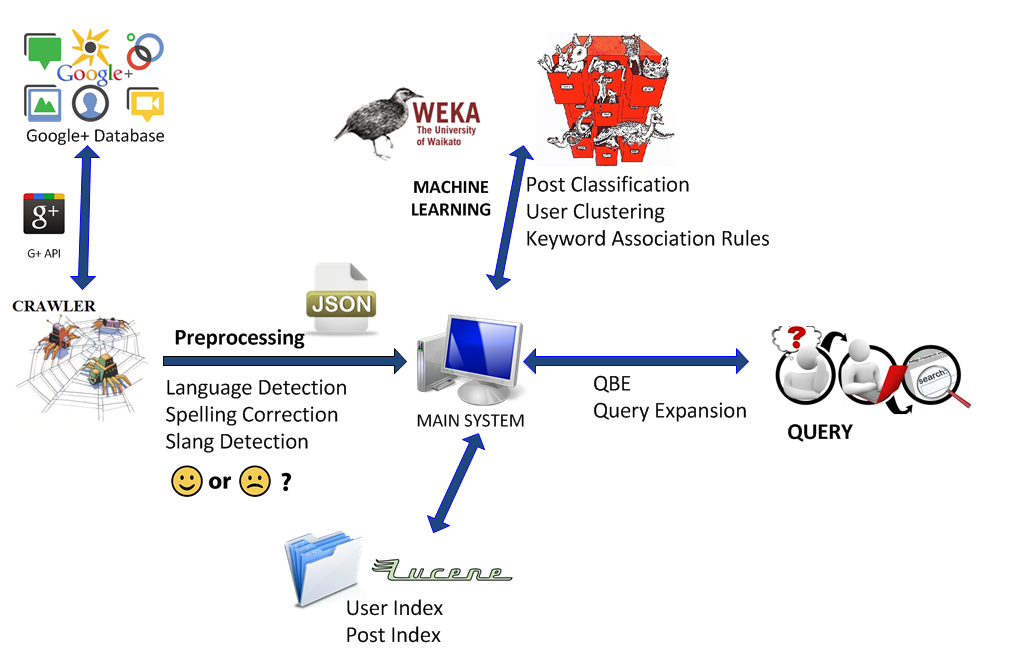
\includegraphics[scale=0.4]{images/architecture.png}
\end{center}
\end{figure}
This Index will be used for searching method.
\item Searching Index
Searching is implemented using Lucene.
\\
Boolean Query
-          OR query is processed by Union in posting list at Lucene indexes.
-          AND query is processed by Intersection in posting list at Lucene indexes.
\\
Scoring Document
In vector space model, user posts are represented in a collection of string vector. For example, a post ��This is a post�� will be represented as string vector (This,is,a,post).
The retrieved user posts are ranked based on how high their score are. Score is calculated using cosine similarity in vector space model.
\end{itemize}

\subsubsection{Evaluation}
The valuation is done manually by giving a query and evaluates the result. Before testing search query, index must be build first. A test query is given by giving a Boolean ��OR��, ��AND��. The query result is listed by their rank and satisfying.


